\documentclass[aspectratio=149]{beamer}

\usepackage[utf8]{inputenc}
\usepackage[T1]{fontenc}

\usepackage[english]{babel}
\usepackage{amsmath}
\usepackage{cleveref}
\usepackage{amssymb}
\usepackage{mathtools}

%%Numbers, expectation
\newcommand{\N}{\mathbb{N}}
\newcommand{\E}{\mathbb{E}}
\renewcommand{\P}{\mathbb{P}}
\newcommand{\Var}{\mathbb{V}}
\newcommand{\R}{\mathbb{R}}
\newcommand{\D}{\mathcal{D}}
\newcommand{\B}{\mathcal{B}}
\newcommand{\Dh}{\D_h}
\renewcommand{\phi}{\varphi}
\newcommand*\diff{\mathop{}\!\mathrm{d}} % integral

%% mathoperator
\DeclareMathOperator*{\argmax}{arg\,max}
\DeclareMathOperator*{\argmin}{arg\,min}
\DeclareMathOperator*{\dom}{dom}
\DeclareMathOperator*{\sign}{sign}
\DeclareMathOperator*{\diag}{diag}

\DeclareMathOperator*{\Cov}{Cov}
\DeclareMathOperator*{\Cor}{Corr}
\DeclareMathOperator*{\Id}{Id}

%proximal operator
\newcommand{\prox}[3][]{\operatorname{prox}^{#1}_{#2}\left(#3 \right)}

\usepackage{xcolor}

%% sort citations by increasing number
\usepackage[sort,nocompress]{cite}

\usepackage{graphicx}% http://ctan.org/pkg/graphicx
\graphicspath{{../figures/}{../../figures}{../../memes}} %Setting the graphicspath
\usepackage{caption,subcaption}

\usepackage{tikz}
\usepackage{pgfplots}
\usetikzlibrary{backgrounds}
\usetikzlibrary{intersections}
\usepgfplotslibrary{fillbetween}

% \usepackage[right]{showlabels}


%%
\theoremstyle{plain}
\newtheorem{prop}{Proposition}[section]
\newtheorem{algo}{Algorithm}[section]
\newtheorem{assumption}{Assumption}
\theoremstyle{remark}
\newtheorem{remark}{Remark}[section]

% cref
\crefname{assumption}{Assumption}{Assumptions}
\crefname{equation}{}{}

\usepackage{autonum}

\usepackage{bm} %% bold math symbols

\usepackage{bbm} %% for \mathbbm{1}


% algorithmic environment
\usepackage{algorithm}
\usepackage[noend]{algpseudocode}

% for some reason this was required on one void linux installation (but not the other)
\usepackage{sansmathaccent}
\pdfmapfile{+sansmathaccent.map}

\author{Axel Böhm}

% shows which section we're in
\usetheme{Darmstadt}

% page number
\setbeamertemplate{footline}[frame number]
\setbeamercolor{page number in head/foot}{fg=gray}


% display things like onslide or visible already before but grayed out
\setbeamercovered{transparent}

% set the itemize item symbol as a diamond
\setbeamertemplate{itemize item}{$\diamond$}
% set the itemize subitem symbol as a triangle
\setbeamertemplate{itemize subitem}{$\blacktriangleright$}

% set the enumerate item symbol as a roman numbers
\setbeamertemplate{enumerate item}{(\roman{enumi})}


\author{Axel Böhm}

% shows which section we're in
\usetheme{Darmstadt}

% page number
\setbeamertemplate{footline}[frame number]
\setbeamercolor{page number in head/foot}{fg=gray}


% display things like onslide or visible already before but grayed out
\setbeamercovered{transparent}

% set the itemize item symbol as a diamond
\setbeamertemplate{itemize item}{$\diamond$}
% set the itemize subitem symbol as a triangle
\setbeamertemplate{itemize subitem}{$\blacktriangleright$}

% set the enumerate item symbol as a roman numbers
\setbeamertemplate{enumerate item}{(\roman{enumi})}


\usepackage{booktabs}

\title{Coordinate descent}
\date{\today}

\begin{document}
\maketitle
\frame{\tableofcontents}


\section{Introduction}%


\begin{frame}
  \frametitle{Coordinate Descent}
  \textcolor{blue}{Goal:} Find $x^* \in \R^d$ minimizing $f(x)$.

  \begin{figure}[ht]
    \centering
    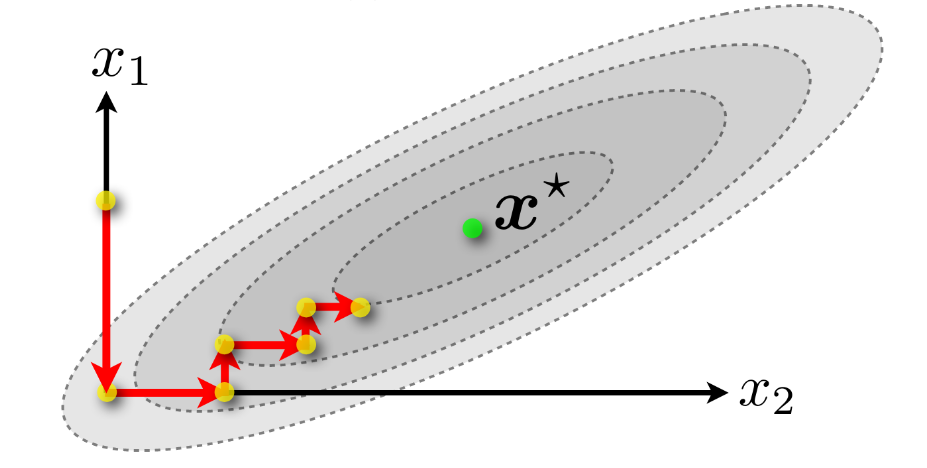
\includegraphics[height=0.7\textheight,keepaspectratio]{coordinate_descent}
    % \caption{\label{fig:label} }
  \end{figure}
  \textcolor{blue}{Observation:} Decrease in function value, but not in distance to solution.
\end{frame}

\begin{frame}
  \frametitle{Coordinate Descent}
  Modify only one coordinate per step:
  \begin{block}{}
    \begin{center}
      select $i_k \in \{1, \dots, d\}$\\
      $x_{k+1} = x_k + \gamma e_{i_k}$
    \end{center}
  \end{block}
  where $e_i$ is the $i$-th unit basis vector.
  Two main variants:
  \begin{itemize}
    \item \textcolor{blue}{Gradient-based stepsize:}
          \begin{equation}
            x_{k+1} = x_k - \frac1L \nabla_{i_k}f(x_k) e_{i_k}
          \end{equation}
    \item \textcolor{blue}{Exact coordinate minimization:} \\
          Solve the \textbf{scalar} problem $\argmin_{\gamma\in \R} f(x_k + \gamma e_{i_k})$.
          \begin{itemize}
            \item \textit{hyperparameter free}
          \end{itemize}
  \end{itemize}
\end{frame}

\section{Randomized coordinate selection}%

\begin{frame}
  \frametitle{Randomized Coordinate Descent}

  \textit{How to choose the coordinate?}

  \begin{block}{}
    \begin{center}
      select $i_k \in \{1, \dots, d\}$ uniformly at random\\
      $x_{k+1} = x_k + \gamma e_{i_k}$
    \end{center}
  \end{block}
  \vspace{1cm}
  \begin{itemize}
    \item \textcolor{blue}{Faster convergence} than gradient descent\\
          (if coordinate step is $d$ times cheaper than full gradient step)
  \end{itemize}
\end{frame}

\begin{frame}
  \frametitle{Technical assumptions}

  \begin{block}{}
    \textcolor{blue}{Coordinate-wise smoothness:}
    \begin{equation}
      f(x + \gamma e_i) \le f(x) + \gamma \nabla_i f(x) + \frac{L}{2}\gamma^2, \quad \forall x \in \R^d, \forall \gamma \in \R, \forall i \in [d]
    \end{equation}
  \end{block}
  Is equivalent to coordinate-wise Lipschitz gradient:
  \begin{equation}
    \vert \nabla_i f(x+ \gamma e_i) - \nabla_i f(x) \vert \le L \vert \gamma \vert.
  \end{equation}

  \begin{itemize}
    \item Additionally we assume \textcolor{blue}{strong convexity}
  \end{itemize}
\end{frame}

\begin{frame}
  \frametitle{Convergence: Linear rate}
  \begin{theorem}
    \label{thm:}
    Let $f$ be coordinate-wise smooth with constant $L$ and $\mu$-strongly convex, then \colorbox{gray!30}{\textup{\texttt{randomized coordinate descent}}} with stepsize $1/L$
    \begin{equation}
      x_{k+1} = x_k - \frac{1}{L} \nabla_{i_k} f(x_k) e_{i_k},
    \end{equation}
    where $i_k \sim Unif(1, \dots, d)$, then
    \begin{equation}
      \E [f(x_k)- f^*] \le {\left(1 - \frac{\mu}{d L}\right)}^k (f(x_0)-f^*).
    \end{equation}
  \end{theorem}
  \textcolor{gray}{Compare to rate of gradient descent.}
\end{frame}

\begin{frame}
  \frametitle{Proof}
  By using smoothness we obtain
  \begin{equation}
    f(x_{k+1}) \le f(x_k) - \frac{1}{2L} \Vert \nabla_{i_k} f(x_k) \Vert^2.
  \end{equation}
  Taking the expectation w.r.t.\ $i$
  \begin{equation}
    \begin{aligned}
      \E [f(x_{k+1})] &\le f(x_k) - \frac{1}{2L} \E[\vert \nabla_{i_k} f(x_k) \vert^2] \\
      &= f(x_k) - \frac{1}{2L}\frac{1}{d} \sum_{i} \vert \nabla_i f(x_k) \vert^2 \\
      &= f(x_k) - \frac{1}{2 d L} \Vert \nabla f(x_k) \Vert^2.\qed
    \end{aligned}
  \end{equation}
  \textcolor{blue}{Lemma:} Strong convexity implies \textcolor{blue}{\textbf{PL}}: $\frac12 \Vert \nabla f(x) \Vert^2 \ge \mu (f(x)-f^*)$
  Therefore, by subtracting $f^*$ on both sides we get the statement of the theorem.
\end{frame}

\begin{frame}
  \frametitle{Polyak-{\L}ojasiewicz (PL) Condition}
  \begin{definition}
    $f$ satisfies the PL condition if the following holds for some $\mu>0$
    \begin{equation}
      \frac12 \Vert \nabla f(x) \Vert^2 \ge \mu (f(x)-f^*).
    \end{equation}
  \end{definition}

  \begin{lemma}%
    Strong convexity implies PL.
  \end{lemma}
  \textcolor{blue}{Proof}
    Strong convexity gives
    \begin{equation}
      f(y) \ge f(x) + \langle \nabla f(x), y-x \rangle + \frac{\mu}{2} \Vert x-y \Vert^2.
    \end{equation}
    Minimizing each side w.r.t. $y$ gives
    \begin{equation}
      f(x^*) \ge f(x) - \frac{1}{2 \mu} \Vert \nabla f(x) \Vert^2. \qed
    \end{equation}
\end{frame}


\begin{frame}
  \frametitle{Linear convergence without strong convexity}
  PL is weaker than strong convexity (doesn't even imply convexity).
  \begin{block}{Examples satisfying PL}
    Let $f := g\circ A$ for strongly convex $g$ and \emph{arbitrary} matrix $A$, \\
    see \textbf{least squares regression}.
  \end{block}

  \begin{corollary}[Linear convergence for PL]%
    Same conditions as before but PL instead of strong convexity yields:
    \begin{equation}
      \E [f(x_k)- f^*] \le {\left(1 - \frac{\mu}{d L}\right)}^k (f(x_0)-f^*).
    \end{equation}
  \end{corollary}
\end{frame}


\section{Other selection rules}%
\label{sec:}

\begin{frame}
  \frametitle{Importance sampling}
  \begin{center}
    \textit{Uniform random selection is not always the best!}
  \end{center}
  \begin{itemize}
    \item Individual smoothness constants $L_i$ for each coordinate $i$
  \end{itemize}
  \begin{equation}
    f(x+ \gamma e_i) \le f(x) + \gamma \nabla_i f(x) + \frac{L_i}{2} \gamma^2
  \end{equation}
  Coordinate descent with selection probabilities $P[i_k=i] = \frac{L_i}{\sum_i L_i}$ and stepsize
  $1/L_{i_k}$ converges with the faster rate
  \begin{equation}
      \E [f(x_k)- f^*] \le {\left(1 - \frac{\mu}{d \bar{L}}\right)}^k (f(x_0)-f^*),
  \end{equation}
  where $\bar{L}= \frac{1}{d} \sum_{i=1}^{d}L_i$. \hfill \textcolor{blue}{Often $\bar{L} \ll L = \max_i L_i$!}
\end{frame}


\begin{frame}
  \frametitle{Steepest Coordinate Descent}
  Selection rule given by
  \begin{equation}
    i_k = \argmax_{i\in [d]} \vert \nabla_i f(x_k) \vert
  \end{equation}
  \emph{``Greedy''}, Gauss-Southwell or \textbf{steepest} coordinate descent.\\
  \textcolor{blue}{Drawback}: requires computation of full gradient if you do not have additional knowledge.
\end{frame}


\begin{frame}
  \frametitle{Convergence of Steepest Coordinate Descent}
  Has same convergence rate as for randomized coordinate descent.\\
  Use the fact that \emph{max} is larger than \emph{average}
  \begin{equation}
    \max_i \vert \nabla_i f(x) \vert^2 \ge  \frac{1}{d} \sum_{i=1}^{d} \vert \nabla_i f(x) \vert^2,
  \end{equation}
  \begin{corollary}%
    \colorbox{gray!30}{\textup{\texttt{steepest coordinate descent}}} with stepsize $1/L$ gives
  \begin{equation}
      f(x_k)- f^* \le {\left(1 - \frac{\mu}{d L}\right)}^k (f(x_0)-f^*).
  \end{equation}
  \end{corollary}
  \textcolor{gray}{Benefit is not clear: more expensive iterations but same bound.}
\end{frame}


\begin{frame}
  \frametitle{Faster Convergence of Steepest Coordinate Descent}
  Faster convergence when measuring strong convexity of $f$ w.r.t $1$-norm instead of the standard Euclidean norm, i.e.
  \begin{equation}
      f(y) \ge f(x) + \langle \nabla f(x), y-x \rangle + \frac{\mu_1}{2} \Vert x-y \Vert_1^2.
  \end{equation}

  \begin{theorem}
    Let $f$ be coordinate-wise smooth with constant $L$ and $\mu_1$-strongly convex, w.r.t. the $1$-norm.
    Then \colorbox{gray!30}{\textup{\texttt{steepest coordinate descent}}} with stepsize $1/L$ yields
    \begin{equation}
      f(x_k)- f^* \le {\left(1 - \frac{\mu_1}{L}\right)}^k (f(x_0)-f^*).
    \end{equation}
  \end{theorem}
  \textcolor{gray}{Compare this to previous contraction factor of $(1-\frac{\mu}{d L})$}.\\
  We always have
  \begin{equation}
    \frac{\mu}{d} \le \mu_1 \le \mu.
  \end{equation}
\end{frame}


\begin{frame}
  \frametitle{Faster Convergence of Steepest Coordinate Descent II}
  \textcolor{blue}{Proof of previous theorem} is same as before, but using the lemma

  \begin{lemma}%
    Let $f$ be $\mu_1$-strongly convex with respect to the $\ell_1$-norm, then
    \begin{equation}
      \frac12 \Vert \nabla f(x) \Vert^2_\infty \ge \mu_1 (f(x)-f^*).
    \end{equation}

  \end{lemma}
\end{frame}

\begin{frame}
  \frametitle{Faster convergence on quadratics}
  \begin{itemize}
    \item If $f$ is a quadratic with diagonal Hessian, we can show
          \begin{equation}
            \mu = \min_i \lambda_i \quad \text{and} \quad \mu_1 = \frac{1}{\sum_{i}^{} \lambda_i}
          \end{equation}
    \item If all $\lambda_i$ are equal:
          \begin{itemize}
            \item No advantage to GS
          \end{itemize}
    \item One very large $\lambda_i$
          \begin{itemize}
            \item GS and random still similar
          \end{itemize}
    \item One very small $\lambda_i$
          \begin{itemize}
            \item GS bound can be much better $\mu_1 \approx \mu$
          \end{itemize}
  \end{itemize}

\end{frame}


\begin{frame}
  \frametitle{Nonsmooth objectives}
  Proved everything for smooth $f$. What about \textcolor{blue}{nonsmooth}?
  \begin{figure}[ht]
    \centering
    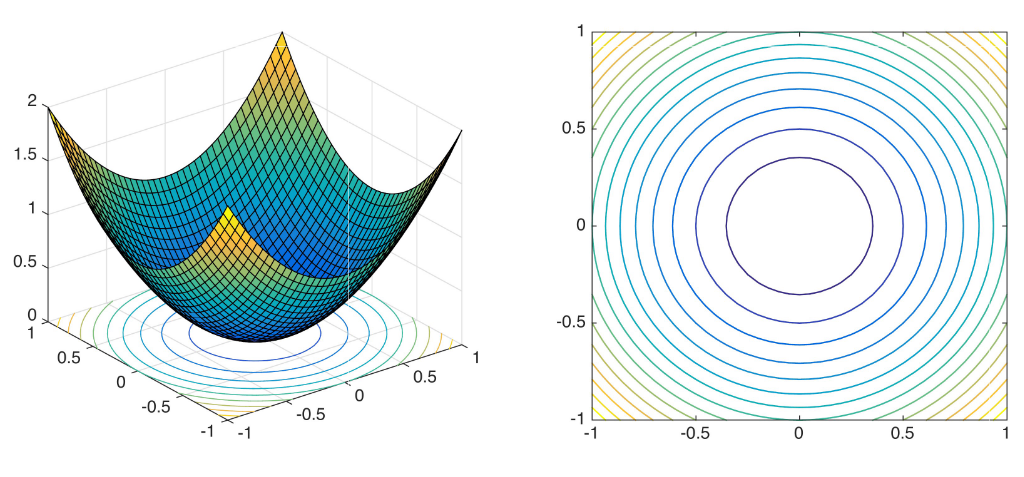
\includegraphics[width=\textwidth,height=\textheight,keepaspectratio]{smooth_function}
    \caption{Example of a smooth function $f(x)= \Vert x \Vert^2$.}
  \end{figure}
\end{frame}


\begin{frame}
  \frametitle{Nonsmooth objectives}
  For general nonsmooth $f$ coordinate descent fails and gets stuck
  \begin{figure}[ht]
    \centering
    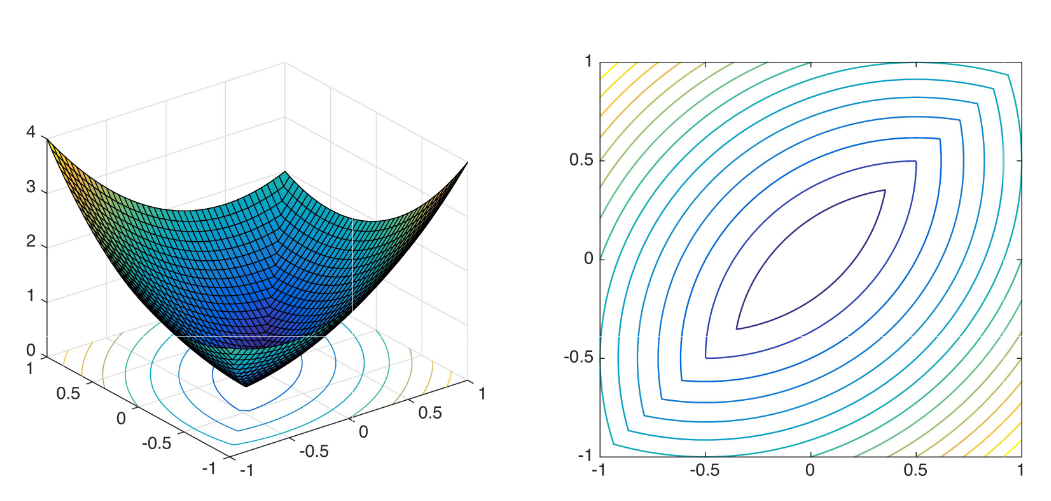
\includegraphics[width=\textwidth,height=\textheight,keepaspectratio]{nonsmooth_function}
    \caption{Example of a nonsmooth function $f(x)= \Vert x \Vert^2 + \vert x_1 - x_2 \vert$.}
  \end{figure}
\end{frame}


\begin{frame}
  \frametitle{Nonsmooth separable objectives}
  If nonsmooth function is \textcolor{blue}{separable} we can get convergence:
  \begin{equation}
    f(x) = g(x) + h(x) \quad \text{with} \quad h(x)= \sum_{i} h_i(x_i)
  \end{equation}
  \begin{figure}[ht]
    \centering
    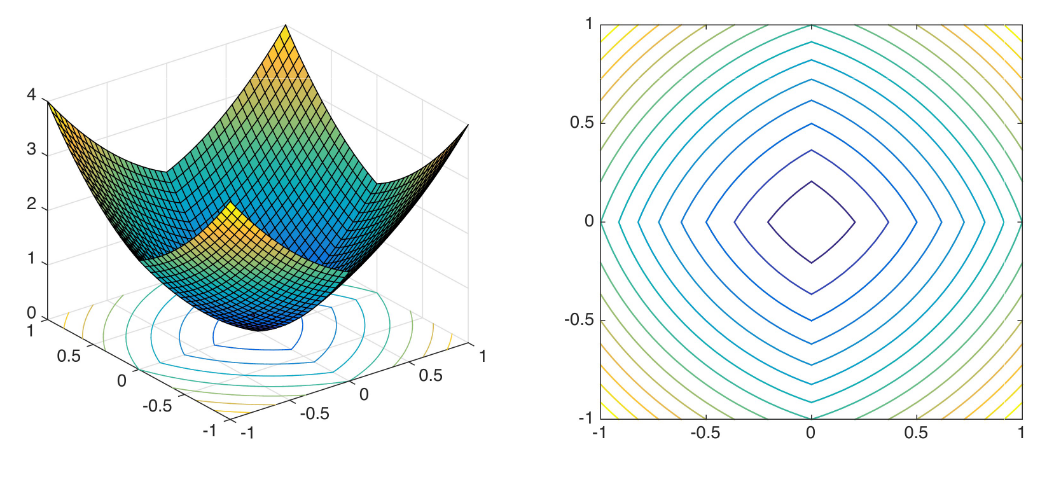
\includegraphics[height=0.5\textheight,keepaspectratio]{nonsmooth_separable}

    \caption{A nonsmooth but separable function $f(x)= \Vert x \Vert^2 + \Vert x \Vert_1$.}
  \end{figure}
\end{frame}




\begin{frame}
  \frametitle{Randomized coordinate descent on non-strongly convex objectives}
  \begin{theorem}
    Let $f$ be coordinate-wise smooth with constant $L$ and convex, then \colorbox{gray!30}{\textup{\texttt{randomized coordinate descent}}} with stepsize $1/L$ yields
    \begin{equation}
      \E [f(x_k)-f^*] \le \frac{2L d \Vert x_0-x^* \Vert^2}{k}
    \end{equation}
  \end{theorem}
  \textcolor{gray}{same observation as in the strongly convex case.}
\end{frame}


\begin{frame}
  \frametitle{Cyclic coordinate descent}
  \begin{theorem}
    Let $f$ be coordinate-wise smooth with constant $L$ then \colorbox{gray!30}{\textup{\texttt{cyclic coordinate descent}}} with stepsize $1/L$ achieves for
    \begin{itemize}
      \item convex objective
            \begin{equation}
              \E [f(x_k)-f^*] \le \frac{4L (d+1) \Vert x_0-x^* \Vert^2}{k}
            \end{equation}
      \item and for $\mu$-strongly convex objectives
            \begin{equation}
              \E [f(x_k)-f^*] \le {\left( 1- \frac{\mu}{2(d+1)L} \right)}^k (f(x_0)-f^*)
            \end{equation}
    \end{itemize}
  \end{theorem}
  \textcolor{gray}{Again, randomized version was better.}
\end{frame}

\begin{frame}
  \frametitle{Some more thoughts}
  \begin{itemize}
    \item minimize all coordinates individually (\textbf{in parallel})
    \item can use blocks of coordinates instead of individual ones
  \end{itemize}

  \textcolor{blue}{State of the art} for generalized linear models $f(x) := g(Ax) + \sum_{i}^{d} h_i(x)$
  \begin{itemize}
    \item Regression, classification (with regularizers)
  \end{itemize}
\end{frame}


\end{document}
